\documentclass[11pt]{article}

\usepackage[margin=1in]{geometry}
\usepackage{graphicx}
\usepackage{xcolor}
\usepackage{booktabs}
\usepackage{caption}
\usepackage{tikz}
\usetikzlibrary{arrows.meta, positioning}
\usepackage[hidelinks]{hyperref}
\usepackage{enumitem}

\definecolor{annblue}{RGB}{50,87,214}
\captionsetup{font=small,labelfont=bf}
\setlength{\parskip}{0.4em}
\setlength{\parindent}{0pt}

\title{\textbf{ANNOT8}\\[2pt]
\large Conversational PDF Annotation with Large Language Models}
\author{Paul Fishwick and Claude Code}
\date{\today}

\begin{document}
\maketitle

\begin{abstract}
\noindent
ANNOT8 is a tool for annotating PDF documents by conversing with a large
language model (LLM). A reader asks questions about a document; each answer is
automatically linked back into the PDF as an Adobe Acrobat-style annotation,
anchored to the passage that supports it. ANNOT8 ships in two forms: a local
Python/Flask application and a fully client-side build hosted on GitHub Pages.
A central design goal is a \emph{copy/paste} mode that lets users of
restricted, enterprise-approved LLMs use the tool with no document data leaving
the browser. This report describes the architecture, the fuzzy quote-location
algorithm that survives OCR noise and LLM page-number drift, and a security
analysis demonstrating zero third-party network egress in the default mode.
\end{abstract}

\section{Introduction and Motivation}

Technical documents---patents, standards, engineering reports---are long and
dense. A reader often wants to interrogate a document and keep the resulting
explanations \emph{attached to the source text}. Conventional workflows split
this in two: one converses with an LLM in one window and annotates the PDF by
hand in another, with no link between the two.

ANNOT8 closes that gap. The user converses with an LLM about a loaded PDF, and
every answer is turned into an annotation placed on the exact passage it draws
from. The work was motivated by a 304-page scanned patent: a document large
enough that manually locating and marking the relevant passages is impractical.

The design goals were: (i) choose among the latest OpenAI, Google, and
Anthropic models; (ii) load a document by drag-and-drop; (iii) offer the
annotation tools of Adobe Acrobat (highlight, comment, shapes); and (iv) work
for enterprise users who may only use a company-approved LLM.

\section{System Architecture}

ANNOT8 has two deployments that share the same workflow and user interface
(Figure~\ref{fig:arch}). The \textbf{local application} is a Python/Flask
backend with a browser frontend; the backend renders pages and writes
annotations with PyMuPDF, performs OCR with Tesseract, and proxies LLM calls.
The \textbf{browser-only build} reimplements the entire pipeline in JavaScript
so it can be hosted as static files on GitHub Pages with no server at all.

\begin{figure}[ht]
\centering
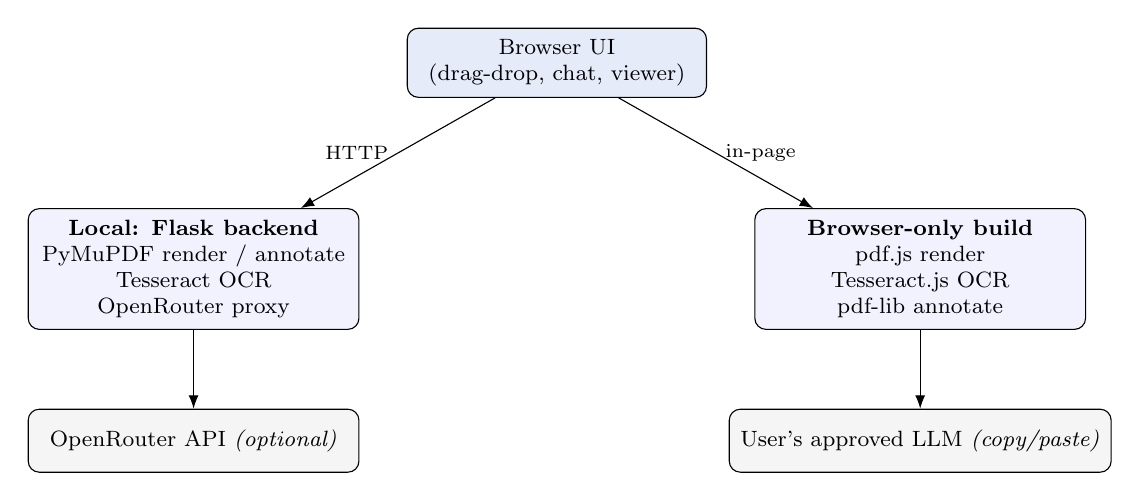
\begin{tikzpicture}[
  font=\footnotesize,
  box/.style={draw, rounded corners, align=center, minimum height=8mm,
              inner sep=4pt},
  comp/.style={box, fill=blue!5},
  title/.style={font=\footnotesize\bfseries}]

  \node[box, fill=annblue!12, minimum width=38mm] (ui) {Browser UI\\
    (drag-drop, chat, viewer)};

  \node[comp, below left=14mm and 6mm of ui, minimum width=42mm] (flask)
    {\textbf{Local: Flask backend}\\ PyMuPDF render / annotate\\
     Tesseract OCR\\ OpenRouter proxy};
  \node[comp, below right=14mm and 6mm of ui, minimum width=42mm] (static)
    {\textbf{Browser-only build}\\ pdf.js render\\ Tesseract.js OCR\\
     pdf-lib annotate};

  \draw[-{Latex}] (ui) -- (flask) node[midway,left,font=\scriptsize]{HTTP};
  \draw[-{Latex}] (ui) -- (static)
    node[midway,right,font=\scriptsize]{in-page};

  \node[box, below=10mm of flask, fill=gray!8, minimum width=42mm] (or)
    {OpenRouter API \emph{(optional)}};
  \node[box, below=10mm of static, fill=gray!8, minimum width=42mm] (cp)
    {User's approved LLM \emph{(copy/paste)}};
  \draw[-{Latex}] (flask) -- (or);
  \draw[-{Latex}] (static) -- (cp);
\end{tikzpicture}
\caption{The two deployments share one UI and workflow. The local build uses
a Flask backend; the browser-only build runs the whole pipeline client-side.}
\label{fig:arch}
\end{figure}

Both builds treat a PDF as a working copy that accumulates annotations, keep
the untouched original separate, and expose the same controls: an LLM-access
mode, a question scope, and an annotation tool.

\section{The Annotation Workflow}

A session begins by dragging a PDF onto the drop zone
(Figure~\ref{fig:dropzone}). The document is opened entirely locally; in the
browser build it is never uploaded anywhere.

\begin{figure}[ht]
\centering
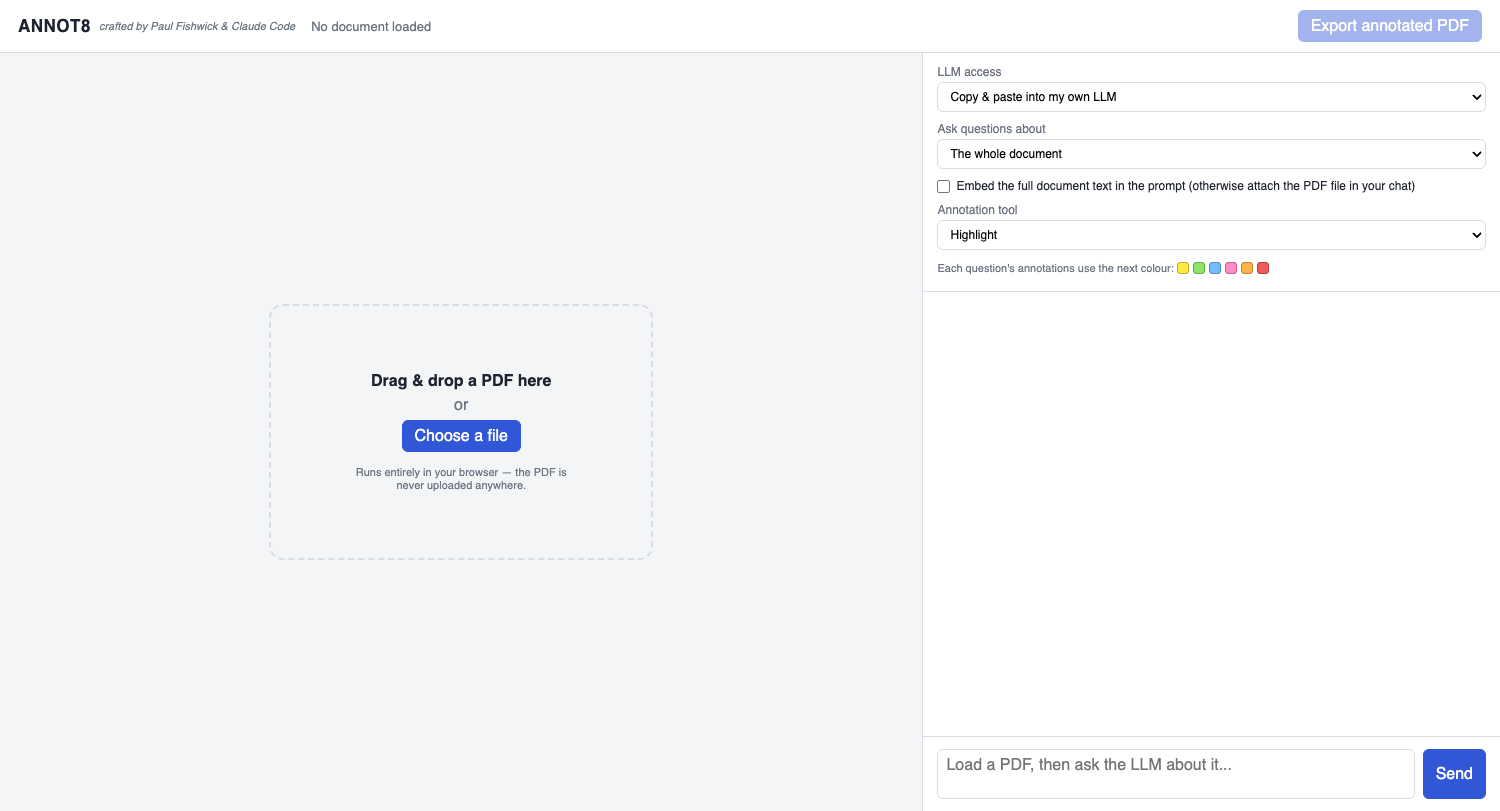
\includegraphics[width=0.86\textwidth]{figures/fig_dropzone.png}
\caption{The ANNOT8 interface on launch. Controls (right) select the LLM
access mode, the question scope, and the annotation tool.}
\label{fig:dropzone}
\end{figure}

The user then chooses a \emph{scope}---the whole document or just the current
page---and asks a question. Each answer is returned in a structured form
containing the prose answer plus a list of \emph{links}: short verbatim
passages, one per key point. ANNOT8 locates each passage in the PDF and applies
the selected annotation. Annotations accumulate across the conversation, and
the highlight colour advances through a six-colour cycle on each question, so
the marks from different questions remain visually distinct
(Figure~\ref{fig:annotated}).

\begin{figure}[ht]
\centering
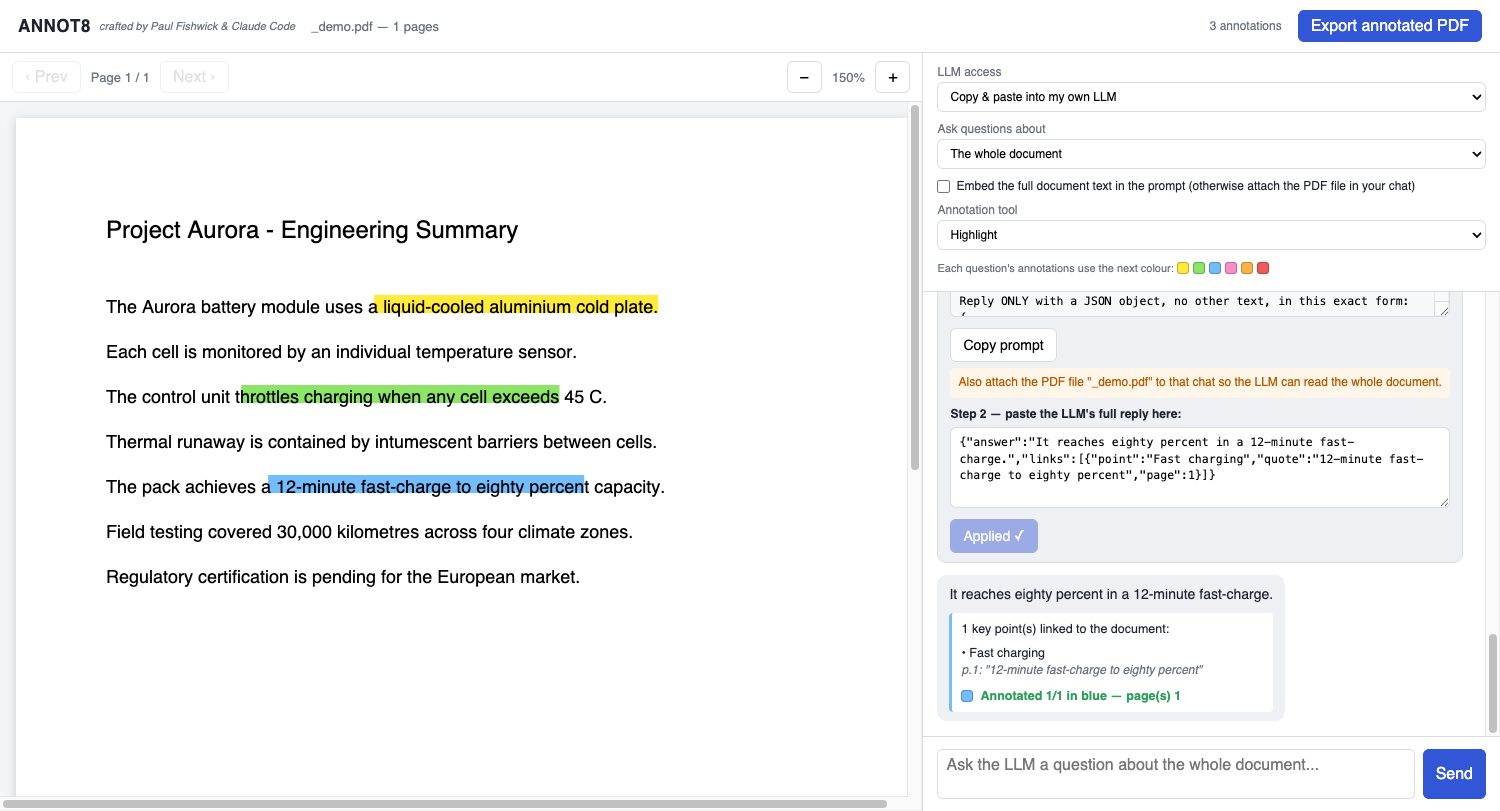
\includegraphics[width=0.96\textwidth]{figures/fig_annotated.png}
\caption{Three questions answered and auto-annotated. Each question's
highlights use the next colour in the cycle (yellow, green, blue); the running
count is shown in the header.}
\label{fig:annotated}
\end{figure}

When finished, the user exports the annotated PDF. The annotations are real PDF
annotation objects, so they appear in Adobe Acrobat's Comments panel with the
LLM's answer as the popup text.

\section{Technical Design}

\subsection{Page Rendering and Text Extraction}

ANNOT8 must recover, for every page, the words and their bounding boxes. It
decides \emph{per page}: if the page has a native text layer it is used
directly (PyMuPDF \texttt{get\_text} or pdf.js \texttt{getTextContent}); if the
page is an image---as in a scanned patent---it falls back to OCR with Tesseract.
The result is cached, and in the local build the whole-document index is also
persisted to disk keyed by a file hash, so re-opening the same PDF skips the
slow OCR pass.

\subsection{Fuzzy Quote Location}

Anchoring an answer to the PDF is the hardest part. The LLM is asked to copy a
verbatim passage and name its page, but in practice both are unreliable: the
page numbers \emph{drift}---on the 304-page patent they were observed off by 39
to 79 pages---and OCR text is never copied character-for-character.

An exact, single-page match therefore fails. ANNOT8 instead uses a fuzzy
matcher. Each word is normalised to a lowercase alphanumeric \emph{content
token}, discarding tokens shorter than three characters so that common words
and single-character OCR noise do not distort the score. A window the size of
the quote is slid across every page of the document; each window is scored by
multiset token overlap with the quote. The best-scoring page wins, with the
LLM's page hint used only to break ties. Within the winning window the
highlight is trimmed to the densest contiguous cluster of matched words, so a
few stray matches elsewhere on the page do not stretch the mark. This survives
OCR errors, word splits, and large page-number drift; on the patent it located
all five summary passages that an exact matcher had missed entirely.

\subsection{Annotation Engine}

ANNOT8 implements the ten annotation tools of Adobe Acrobat's markup set:
highlight, underline, strikethrough, squiggly underline, sticky note, text
box, callout, rectangle, oval, and arrow. In the local build these are written
with PyMuPDF; in the browser build with pdf-lib, constructing the PDF
annotation dictionaries directly. Six highlight colours are available and are
cycled per question. Every annotation stores the LLM's answer as its
\texttt{Contents}, so it is readable in any PDF viewer's comment list.

\subsection{LLM Access Modes}

Two ways of reaching an LLM are offered. In \textbf{OpenRouter API mode} the
application calls the OpenRouter API directly, using the latest Claude, GPT,
and Gemini models. In \textbf{copy/paste mode}---the default---ANNOT8 builds a
self-contained prompt and displays it for the user to copy
(Figure~\ref{fig:promptcard}). The user pastes it into their own LLM chat,
then pastes the reply back into ANNOT8, which parses it and annotates the PDF.
For a whole-document question the user may either embed the document text in
the prompt or simply attach the PDF file in their chat.

\begin{figure}[ht]
\centering
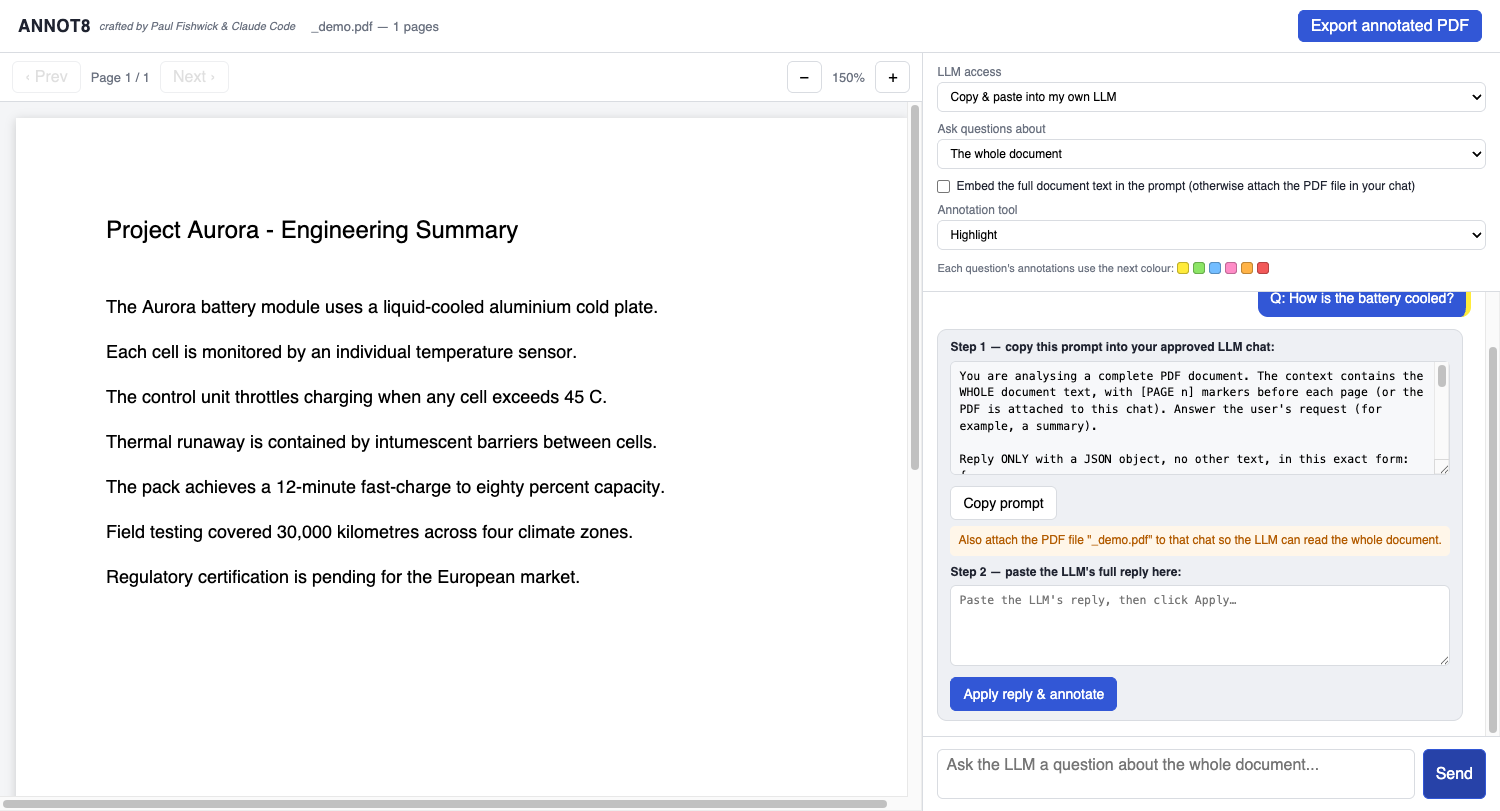
\includegraphics[width=0.96\textwidth]{figures/fig_promptcard.png}
\caption{Copy/paste mode. ANNOT8 generates a prompt for the user to paste into
their own approved LLM; the reply is pasted back and applied locally.}
\label{fig:promptcard}
\end{figure}

Copy/paste mode exists precisely so that a user restricted to a
company-approved LLM can still use ANNOT8: the human uses the sanctioned chat
interface directly, and ANNOT8 acts only as a helper around it.

\section{The Browser-Only Build}

The GitHub Pages build (in the repository's \texttt{docs/} folder) runs the
entire pipeline in the browser: pdf.js renders pages and reads native text,
Tesseract.js performs OCR, pdf-lib writes the annotations, and the fuzzy
matcher is ported to JavaScript. All libraries are \emph{vendored} into the
site rather than loaded from a content-delivery network, so the application
works offline and behind corporate proxies that block external CDNs. It is
live at \url{https://metaphorz.github.io/annot8/}.

\section{Security and Data-Leak Analysis}

A core requirement is that for an enterprise user with a private, proprietary
LLM, \emph{nothing the user enters may leak}. This section reports an audit of
the browser-only build against that requirement.

\textbf{Code audit.} The only outbound HTTP request issued by ANNOT8's own
code is the OpenRouter call, and it executes only in API mode. There is no
\texttt{XMLHttpRequest}, no WebSocket, no analytics or telemetry, and every
library is served from the application's own origin.

\textbf{Empirical network capture.} A full session was driven with Selenium
while recording every network request the browser made. The results
(Table~\ref{tab:net}) confirm that in the default copy/paste mode, once the
page has loaded, ANNOT8 makes \emph{no} network requests at all---and that OCR
of a scanned page contacts no external host.

\begin{table}[ht]
\centering
\small
\begin{tabular}{lll}
\toprule
\textbf{Session} & \textbf{Requests} & \textbf{External hosts} \\
\midrule
Copy/paste: load, ask, paste reply, annotate, export & 8 (all own host) & none \\
Scanned-patent load + in-browser OCR of a page & 10 (all own host) & none \\
\bottomrule
\end{tabular}
\caption{Every network request observed during full sessions. In copy/paste
mode there is zero third-party traffic.}
\label{tab:net}
\end{table}

\textbf{Why copy/paste mode does not leak.} The PDF is read into memory with
the browser's \texttt{FileReader} and processed entirely in-page. The prompt is
placed in a text box for the user to copy; ANNOT8 never transmits it. The user
pastes it into their own LLM, through their own approved channel; the reply is
parsed and applied locally; the annotated PDF is generated and downloaded
locally. Browser \texttt{localStorage} holds only the chosen mode and an
optional API key, and is never transmitted.

\textbf{Vendored OCR.} Tesseract's engine, WebAssembly core, and English
language data are all vendored, so OCR of a scanned document downloads nothing
and uploads nothing---OCR runs locally in WebAssembly.

\textbf{Residual considerations.} Three points are disclosed honestly. First,
loading the page from GitHub Pages is a request to GitHub; an enterprise can
eliminate this by self-hosting the static \texttt{docs/} folder on an internal
server (see \texttt{SELF-HOSTING.md}). Second, OpenRouter API mode \emph{does}
send document text to a third party and must not be used for proprietary
material---the default copy/paste mode is the safe one. Third, once the user
pastes content into their own LLM, that data travels through their approved
channel, which is outside ANNOT8's control and the user's own responsibility.

\section{Validation and Testing}

ANNOT8 is covered by automated tests, with browser behaviour exercised through
Selenium as required for asynchronous, LLM-driven interfaces. The Flask backend
passes 29 of 29 checks, the local UI 9 of 9, and the browser-only build 10 of
10---including loading a PDF, the copy/paste flow, colour cycling, and an
exported file verified to carry its annotations.

End to end, a whole-document summary of the 304-page patent produced five key
points, all five located and highlighted despite page-number drift of up to 79
pages. Figure~\ref{fig:patent} shows annotations placed on the patent's claims.

\begin{figure}[ht]
\centering
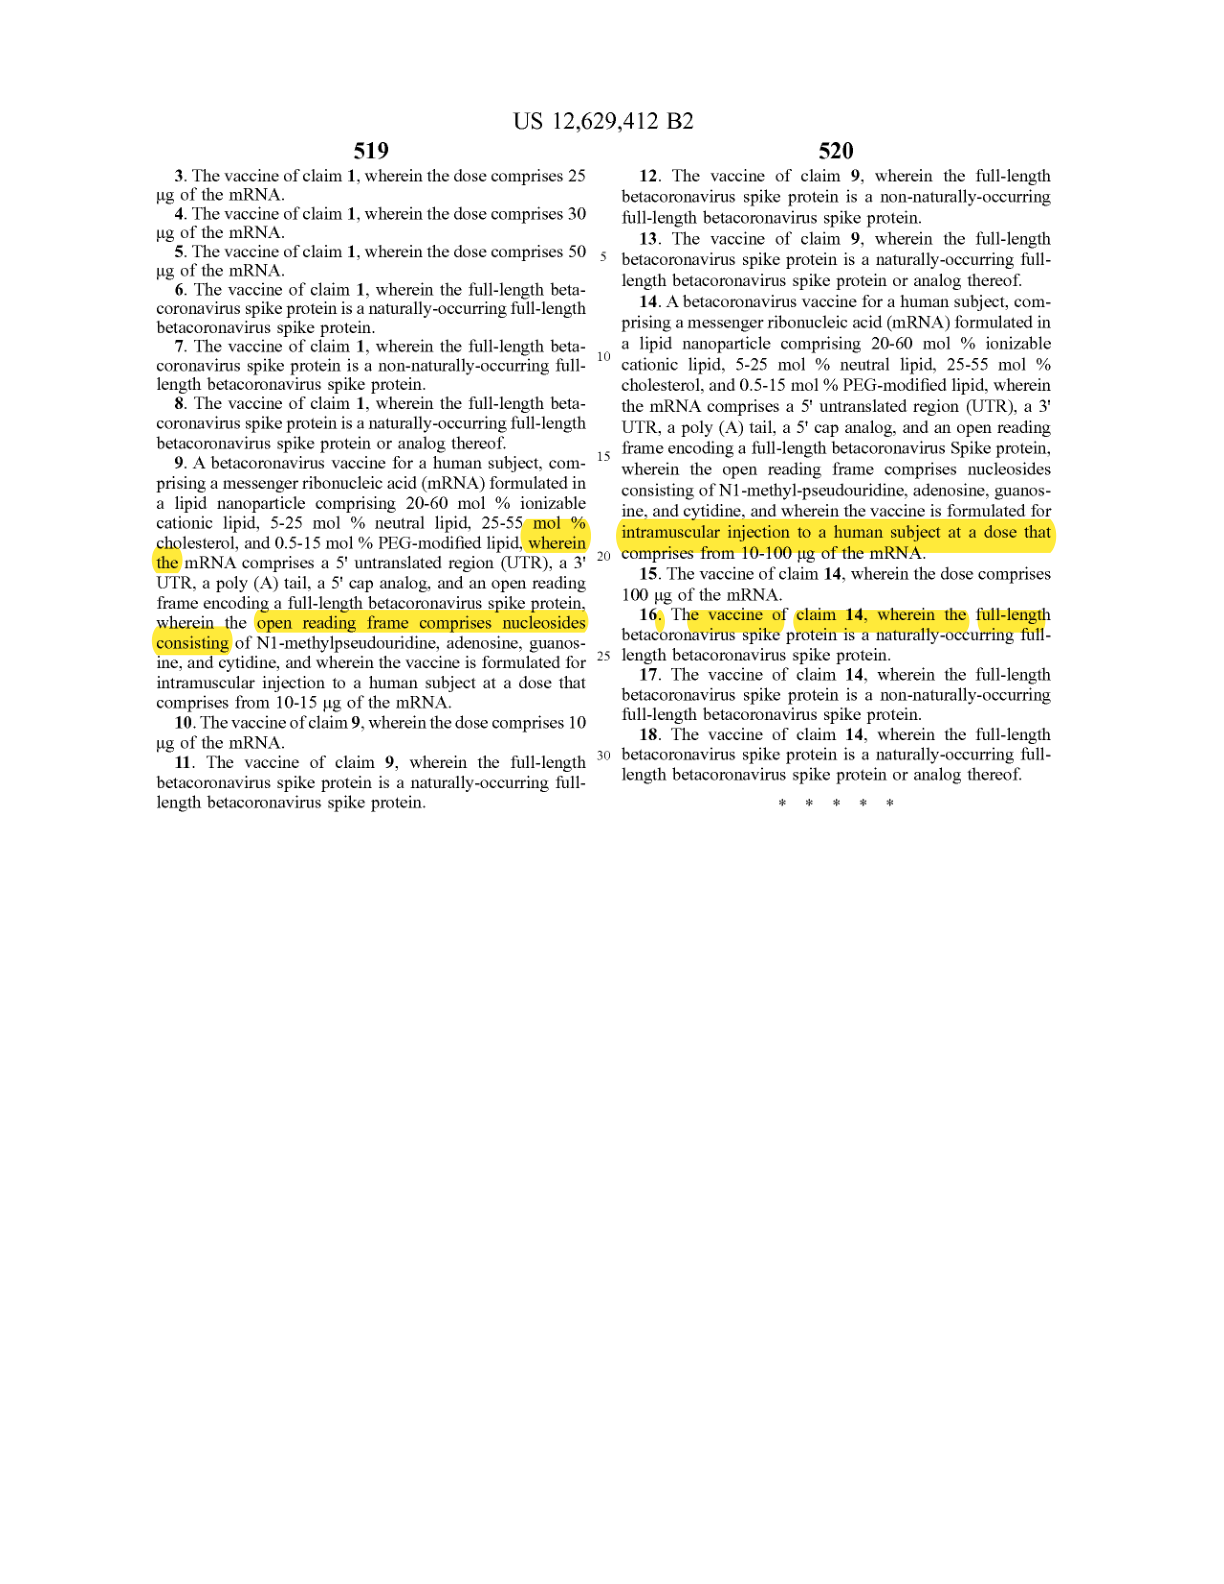
\includegraphics[width=0.74\textwidth]{figures/fig_patent.png}
\caption{Annotations placed on a page of the 304-page scanned patent. The
passages were located by OCR and the fuzzy matcher, not by the page numbers
the LLM supplied.}
\label{fig:patent}
\end{figure}

\section{Conclusion and Future Work}

ANNOT8 turns a conversation with an LLM into a set of source-anchored PDF
annotations, in both a local application and a server-free build suitable for
GitHub Pages. Its fuzzy matcher makes automatic anchoring robust to OCR noise
and unreliable LLM page numbers, and its copy/paste mode lets enterprise users
benefit from the tool without document data leaving the browser---a property
verified by network capture, not merely asserted.

Future work includes fully vendoring additional OCR language models, extending
the matcher with order-aware scoring for paraphrased quotes, and an in-app
index of annotated pages for navigation without a separate PDF viewer.

\vspace{1em}
\hrule
\vspace{0.5em}
\small\noindent
\textit{ANNOT8 --- crafted by Paul Fishwick and Claude Code.}
Source: \url{https://github.com/metaphorz/annot8}

\end{document}
